\subsubsection{Common Spatial Patterns}
Common Spatial Patterns (CSP)\nomenclature{CSP}{Common Spatial Patterns} is a supervised technique that has its origin in the optimization of motor imagery BCIs\citep{CSPSeba}. It is a common technique in BCI research\cite{ErrorPotentials,svmldacomp,currTrends}. CSP creates linear combinations of the original EEG channels that maximize the variance for one class while simultaneously minimizing the variance of the other class \cite{ErrorPotentials}. One disadvantage of using CSP is that the default version can only distinguish between 2 classes, though one can easily aggregate multiple CSP models to create one-vs-one and one-vs-all models, similarly to the one-vs-one and one-vs-all SVMs.

\npar

The input for a CSP filter is a set of N labelled samples $E_j (j=1...N)$, with dimension $N_{ch}$ x $T_j$, with $N_{ch}$ being the number of EEG channels and $T_j$ the number of samples in a single trial\citep{CSPSeba}.

\npar

First the train data is split into two classes, before computing the covariance matrices of both classes.
\begin{center}
$\Sigma_1 = {\displaystyle \sum_{j \in C_1}} X\frac{E_jE_j^T}{trace(E_jE_j^T)}$ \\
$\Sigma_2 = {\displaystyle \sum_{j \in C_2}} X\frac{E_jE_j^T}{trace(E_jE_j^T)}$ \\
\end{center}
Note that the average of $E_j$ is expected to be zero, because a bandpass filter is applied that makes the DC component of the signal zero. The next step is to calculate the composite covariance matrix.
\begin{center}
$\Sigma = \Sigma_1 + \Sigma2$
\end{center}

\npar

Next the covariance matrix is diagonalised by calculating the eigenvalues and eigenvectors of $\Sigma$.
\begin{center}
$V^T\Sigma V = P$
\end{center}
The eigenvalues are then found on the diagonal of P, each eigenvalue corresponds to an eigenvector found in the columns of V.

\npar

The next step is the whitening transformation.
\begin{center}
$U = P^{\frac{1}{2}}V^T$ \\
\end{center}
Which results in
\begin{center}
$U\Sigma U^T = 1$
\end{center}
Next the following two matrices are calculated:
\begin{center}
$R_1 = U\Sigma_1U^T$\\
$R_2 = U\Sigma_2U^T$
\end{center}
$R_1$ is then diagonalised
\begin{center}
$Z^TR_1Z = D = diag(d1, ..., d_m)$
\end{center}
The eigenvalues on the diagonal are then sorted, as larger eigenvalues correspond to higher importances. %TODO
Next the filters are determined by:
\begin{center}
$W = Z^TU$
\end{center}
The EEG channels can then be filtered as follows:
\begin{center}
$E^{CSP} = WE^{orig}$
\end{center}

\npar

Since CSP filters create simple linear combination of incoming channels, they can also be used as feature selection mechanism,albeit in a limited fashion. The result of a CSP transformation are again a set of EEG channels, where each channel is a combination of the previous channels. The first and last row of the resulting matrix $W$ shows the coefficients for which the variance is maximized between the two signals. Looking at those coefficients, one can determine which channels are of more importance than other and thus which channel locations have the most influence on emotion.



%TODO opkuisen
Machine learning can be used for emotion recognition to find patterns in features extracted from physiological signals\citep{DEAP,ExtendedPaper}. The output of the machine learning algorithm is a prediction of the subject's emotional state. The general process of machine learning is as follows, the process starts with gathering EEG data, from which features are extracted. These features are then fed to a machine learning algorithm, which outputs a prediction. This is shown in Figure \ref{eegtopred}

\mijnfiguur{width=0.9\textwidth}{eegtopred}{The basic setup for emotion recognition with machine learning. In the first step, physiological signals are gathered. Next: features are extracted and passed to a machine learning algorithm. The output of the machine algorithm is a prediction of the emotional state, in the valence/arousal space. }

To recognise emotion in the brain, features need to be extracted from the physiological signals. In this thesis, two categories of physiological features are observed: non-EEG features and EEG features. Non-EEG features are physiological signals like heart rate, skin conductivity, respiration rate, etc. EEG features, on the other hand, are features extracted from the EEG measurements of the subjects. 


\section{Important EEG channels}

Another component of this work is to dig into the EEG features and find out which channels are most important. This was done by taking the Random forest as a feature selection model and looking at the models that were build. By simply counting the occurrences of different EEG channels in these models, pie charts were constructed. This was done for both valence and arousal. The results are displayed in Figure\ref{arousalchannel} for arousal and Figure \ref{valencechannel} for valence.


\mijnfiguur{width=1.\textwidth}{arousal_psd.eps}{todo}
\mijnfiguur{width=1.\textwidth}{valence_psd.eps}{todo}


\begin{figure}[H]
\centering
  \begin{subfigure}[b]{.5\textwidth}
    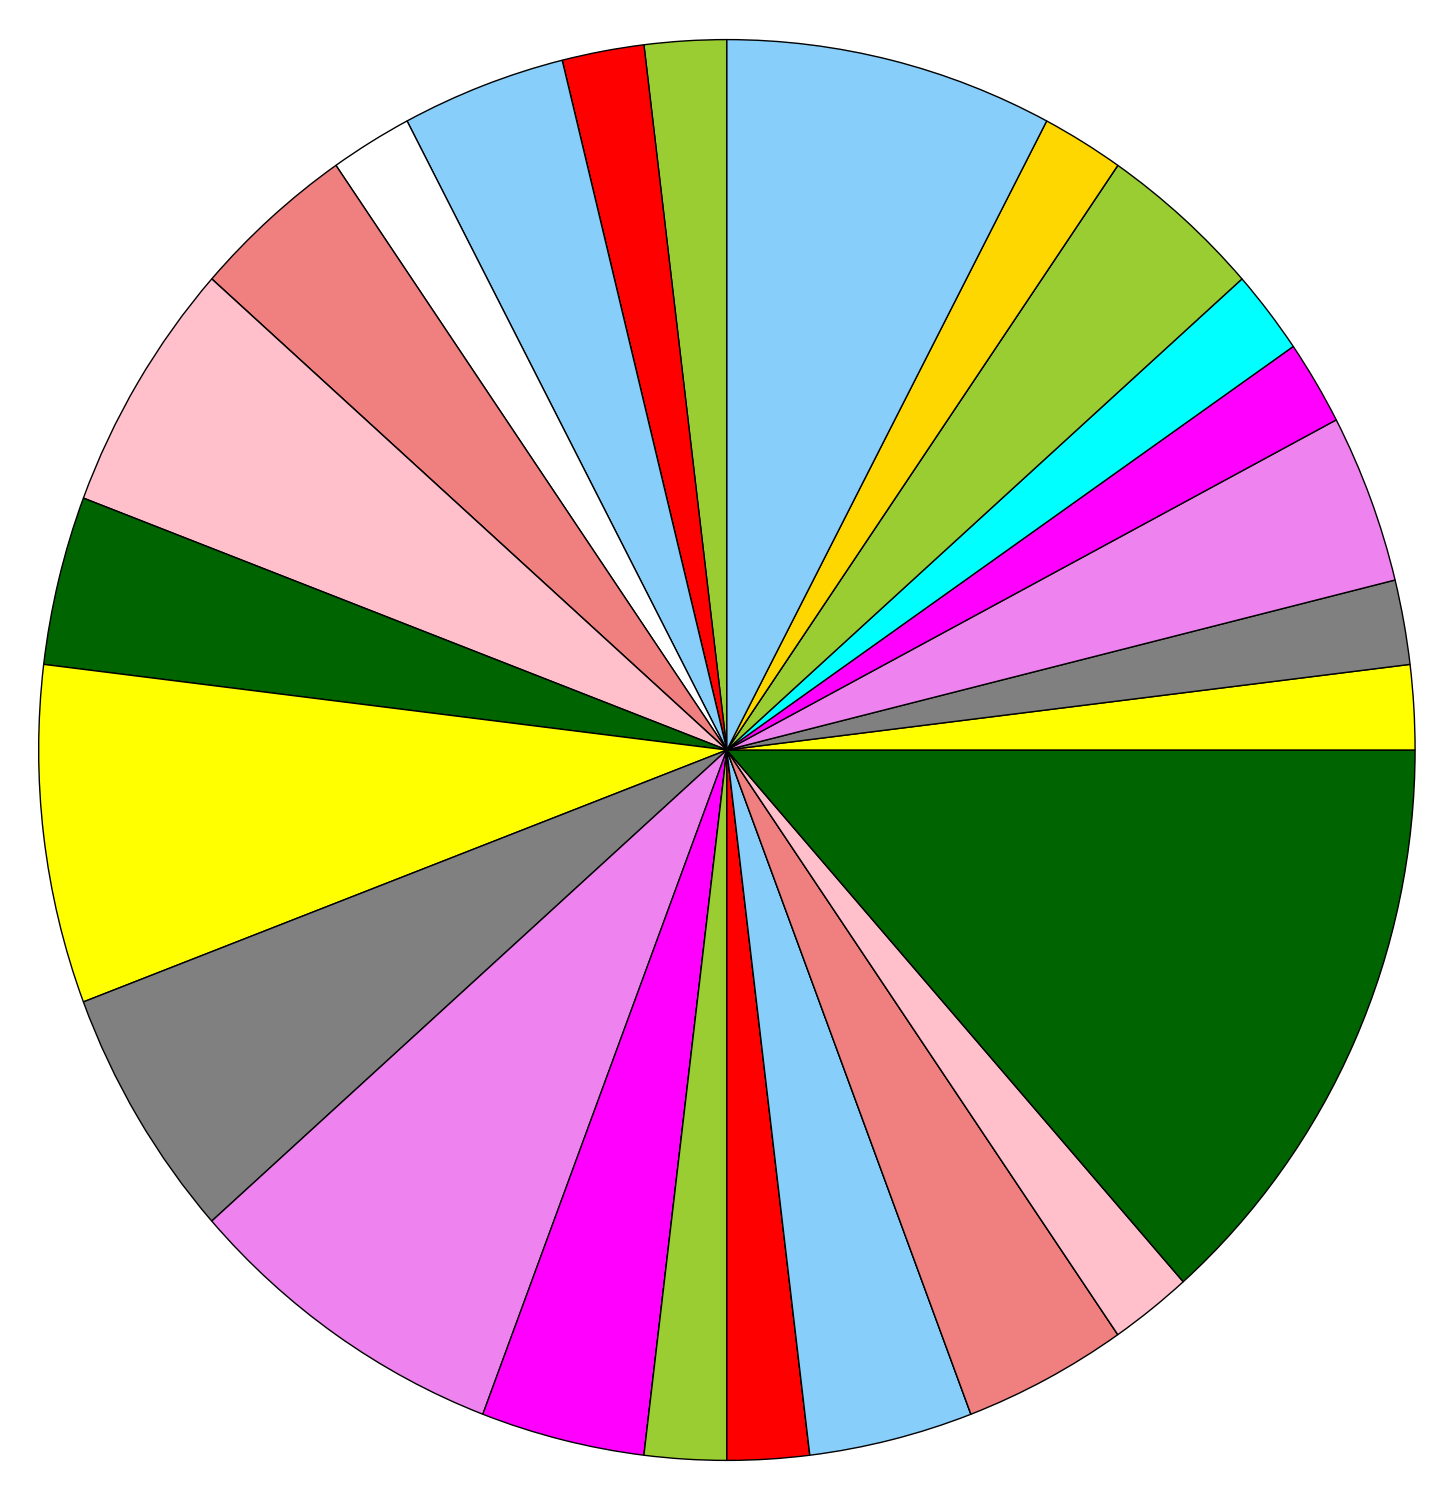
\includegraphics[width=\textwidth]{arousalchannel}
    \caption{The different selected channels for arousal.\label{arousalchannel}}
  \end{subfigure}
\hfill
  \begin{subfigure}[b]{.4\textwidth}
    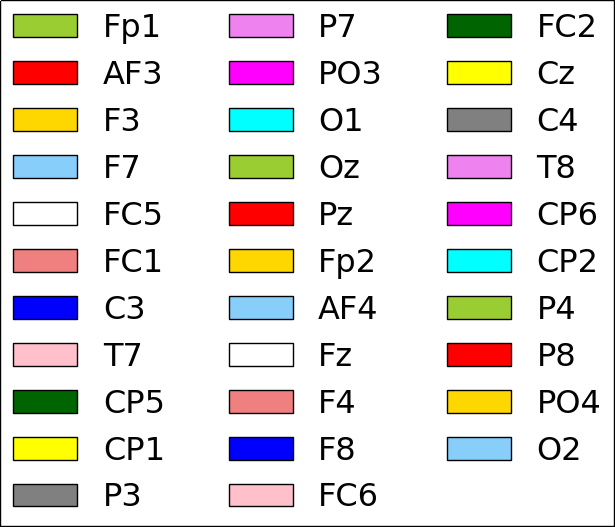
\includegraphics[width=\textwidth]{channellegend}
    \caption{Each color and its corresponding EEG channel.}
  \end{subfigure}
\end{figure}

\begin{figure}[H]
\centering
  \begin{subfigure}[b]{.5\textwidth}
    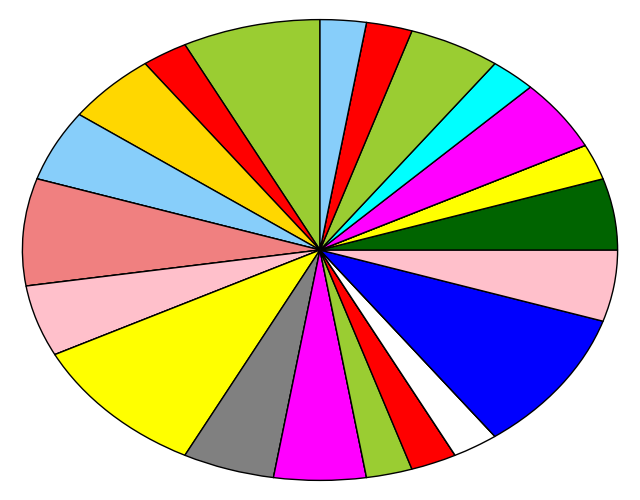
\includegraphics[width=\textwidth]{valencechannel}
    \caption{The different selected channels for valence.\label{valencechannel}}
  \end{subfigure}
\hfill
  \begin{subfigure}[b]{.4\textwidth}
    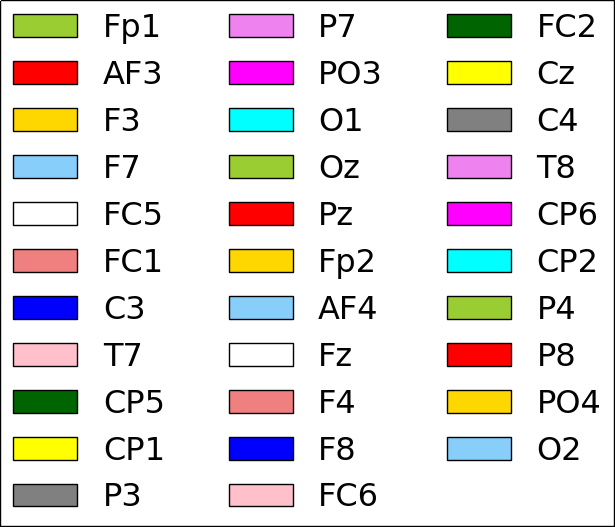
\includegraphics[width=\textwidth]{channellegend}
    \caption{Each color and its corresponding EEG channel.}
  \end{subfigure}
\end{figure}

At first it seems that there is no agreement on the channels, one possible reason for this, might be that electrodes are not placed exactly. Even though the 10/20 system defines the different locations quite well, it is still possible that small variations in the locations exists. Grouping the channels might give a more clear view of the important regions of the brain. The channels were grouped as follows: 
\begin{table}[H]
\centering
\caption{The region for each EEG channel}
\begin{tabular}{ll|ll|ll|ll}
\textbf{Channel} & \textbf{Region} & \textbf{Channel} & \textbf{Region} & \textbf{Channel} & \textbf{Region}      & \textbf{Channel} & \textbf{Region}     \\ \hline
\textbf{Fp1}     & front left      & \textbf{CP5}     & back left       & \textbf{Fp2}     & front right & \textbf{C4}      & back right \\
\textbf{AF3}     & front left      & \textbf{CP1}     & back left       & \textbf{AF4}     & front right & \textbf{T8}      & back right \\
\textbf{F3}      & front left      & \textbf{P3}      & back left       & \textbf{Fz}      & midline     & \textbf{CP6}     & back right \\
\textbf{F7}      & front left      & \textbf{P7}      & back left       & \textbf{F4}      & front right & \textbf{CP2}     & back right \\
\textbf{FC5}     & front left      & \textbf{PO3}     & back left       & \textbf{F8}      & front right & \textbf{P4}      & back right \\
\textbf{FC1}     & front left      & \textbf{O1}      & back left       & \textbf{FC6}     & front right & \textbf{P8}      & back right \\
\textbf{C3}      & back left       & \textbf{Oz}      & midline         & \textbf{FC2}     & front right & \textbf{PO4}     & back right \\
\textbf{T7}      & back left       & \textbf{Pz}      & midline         & \textbf{Cz}      & midline     & \textbf{O2}      & back right
\end{tabular}
\end{table}

These Region are also depicted in Figure \ref{regions}.
\mijnfiguur{width=.8\textwidth}{regions}{All EEG channels were grouped in 4 regions: left-front (blue), right-front (red), left-back(black), right-back (purple) and midline (yellow).}

The resulting distributions are shown in Figure \ref{arousalzones} for arousal and in Figure \ref{valencezones}, the legend is shown in Figure \ref{zonelegend}.

\begin{figure}[H]
\centering
  \begin{subfigure}[b]{.4\textwidth}
    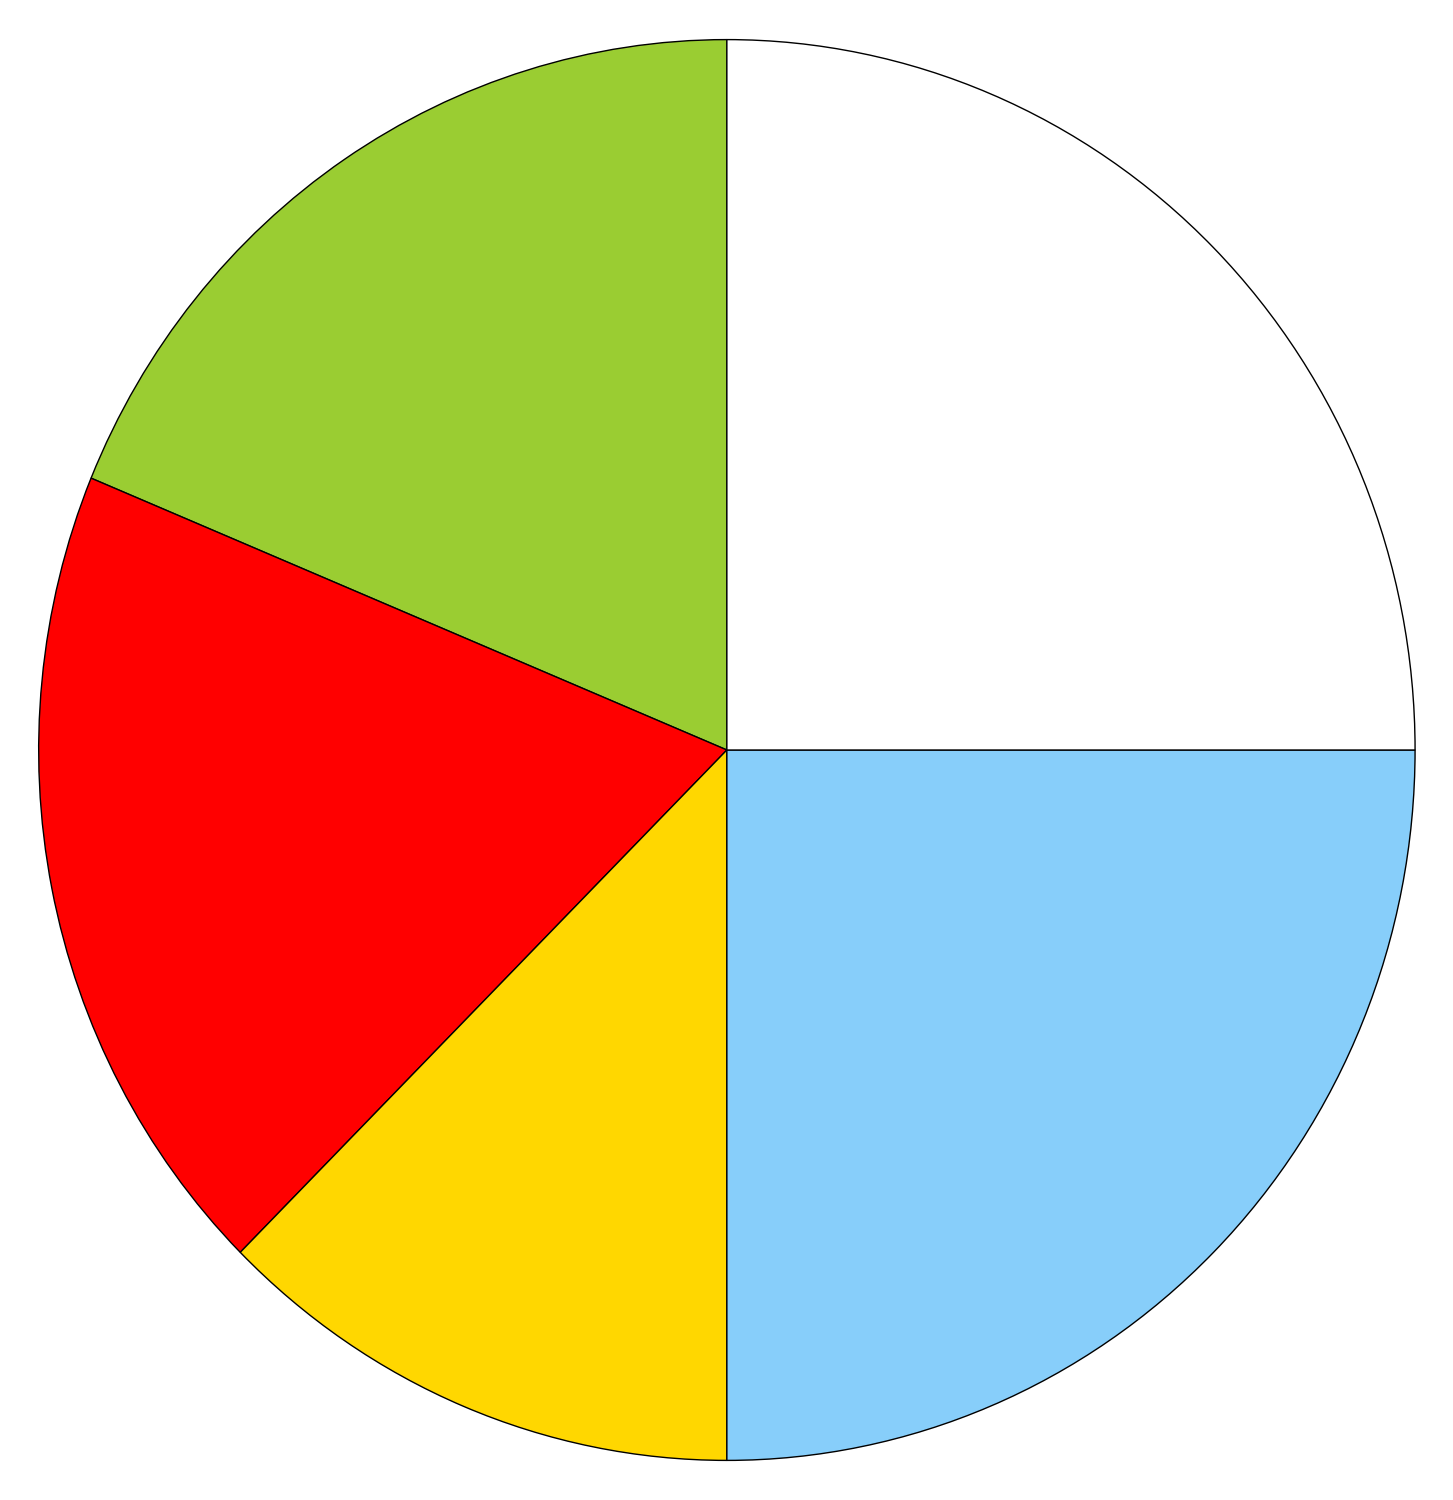
\includegraphics[width=\textwidth]{arousalzones}
    \caption{Origin of the power features for arousal classification.\label{arousalzones}}
  \end{subfigure}
\hfill
  \begin{subfigure}[b]{.4\textwidth}
    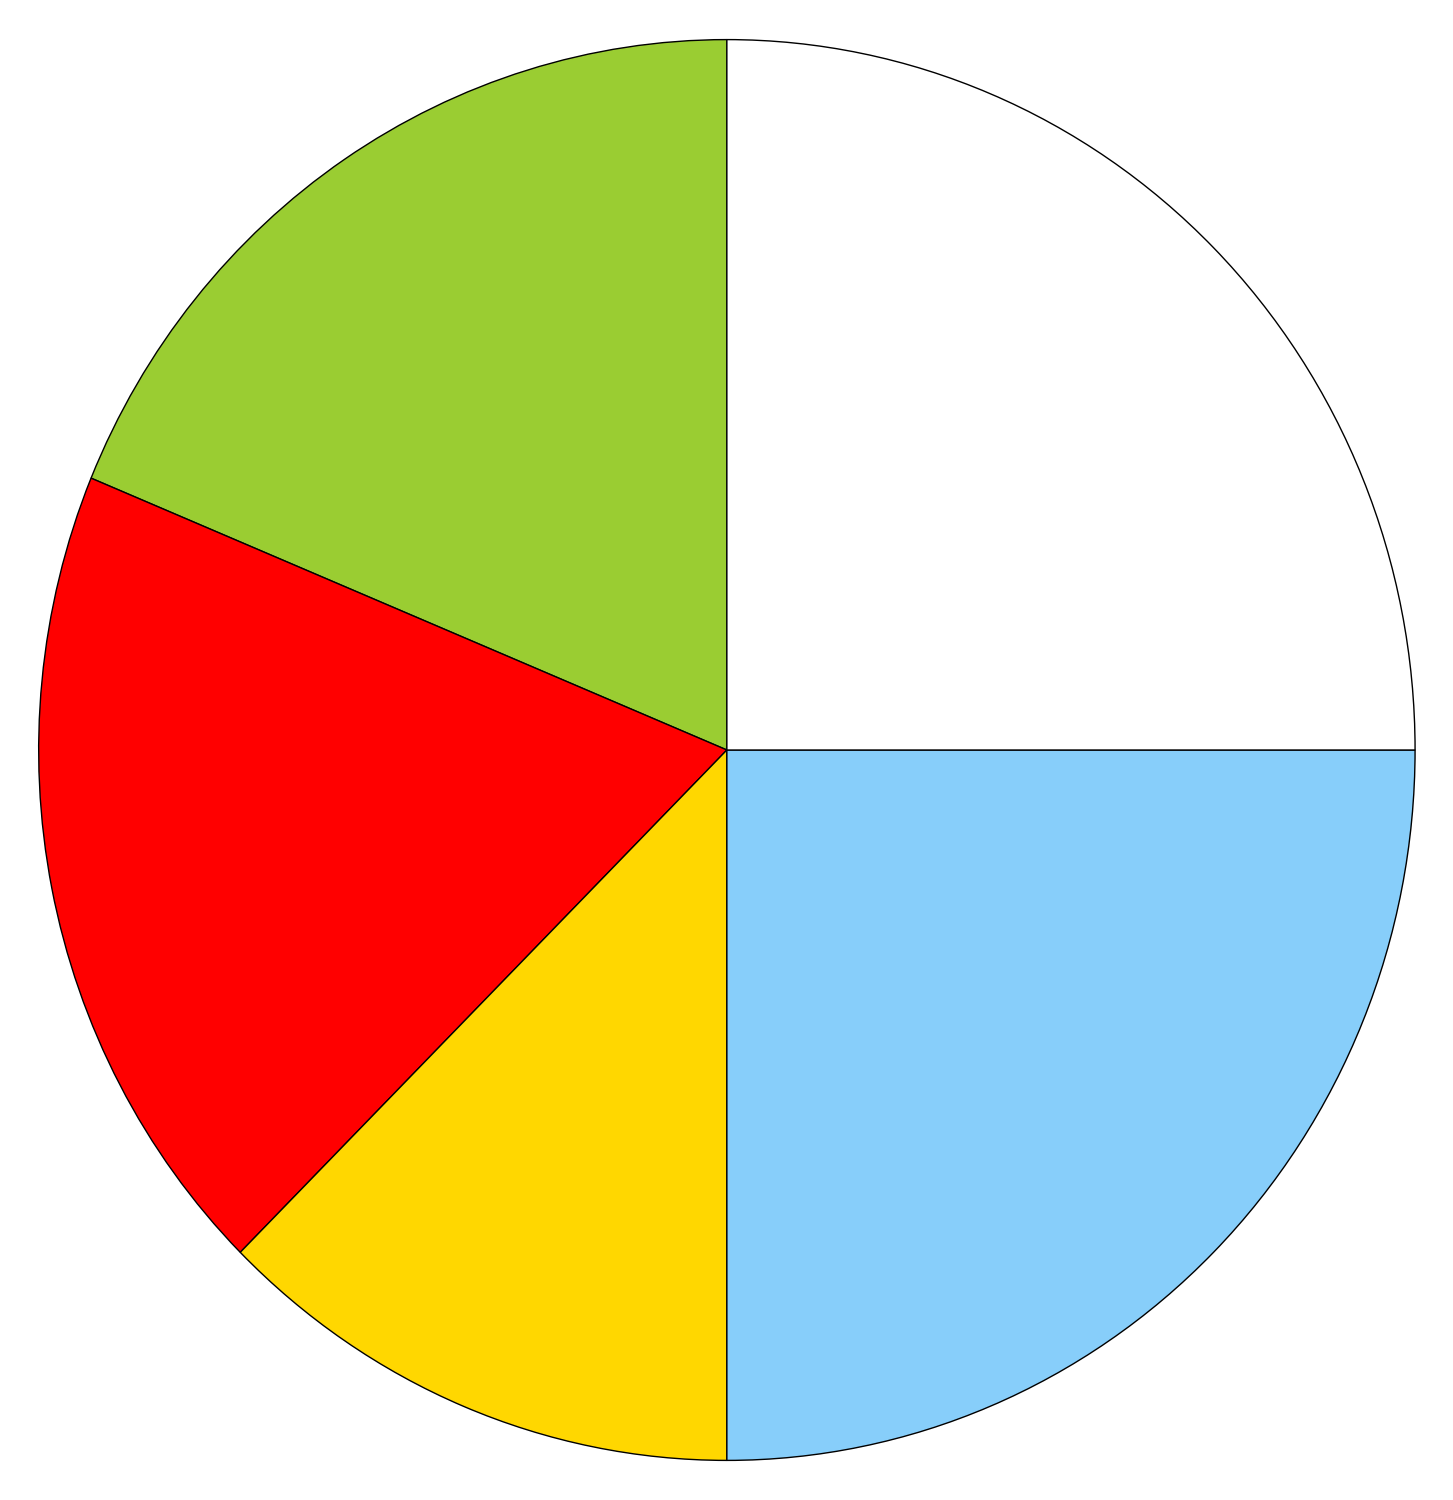
\includegraphics[width=\textwidth]{valencezones}
    \caption{Origin of the power features for valence classification.\label{valencezones}}
  \end{subfigure}
\\
  \begin{subfigure}[b]{.7\textwidth}
    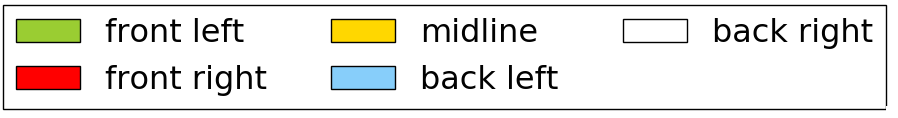
\includegraphics[width=\textwidth]{zonelegend}
    \caption{The corresponding zone for each color.\label{zonelegend}}
  \end{subfigure}
\end{figure}

Looking at the pie plots, one can see that there is no clear region used. The back left and right regions appear most often, but the difference with the front left and right is little. It seems that for both valence and arousal, power values of all different regions might be of importance. The distributions for the regions are the same for both valence and arousal, but they differ in terms of channels.

\npar

The same principle can be done for the asymmetry features, here a distinction was made between DASM and RASM features on one hand and the DCAU and RCAU features on the other hand. The DASM and RASM features were divided in channel pairs located at the front and back of the brain. A specific list is given in Table \ref{ASMgroupTable} below.

%table
\begin{table}[H]
\centering
\caption{the region for each DASM and RASM channel pair\label{ASMgroupTable}}
\begin{tabular}{ll|ll}
\textbf{Channel pair} & \textbf{Group} & \textbf{Channel pair} & \textbf{Group} \\ \hline
Fp1,Fp2               & front          & C3,C4                 & back           \\
AF3,AF4               & front          & T7,T8                 & back           \\
F3,F4                 & front          & CP5,CP6               & back           \\
F7,F8                 & front          & CP1,CP2               & back           \\
FC5,FC6               & front          & P3,P4                 & back           \\
FC1,FC2               & front          & P7,P8                 & back           \\
                      &                & PO3,PO4               & back          
\end{tabular}
\end{table}

\begin{figure}[H]
\centering
  \begin{subfigure}[b]{.4\textwidth}
    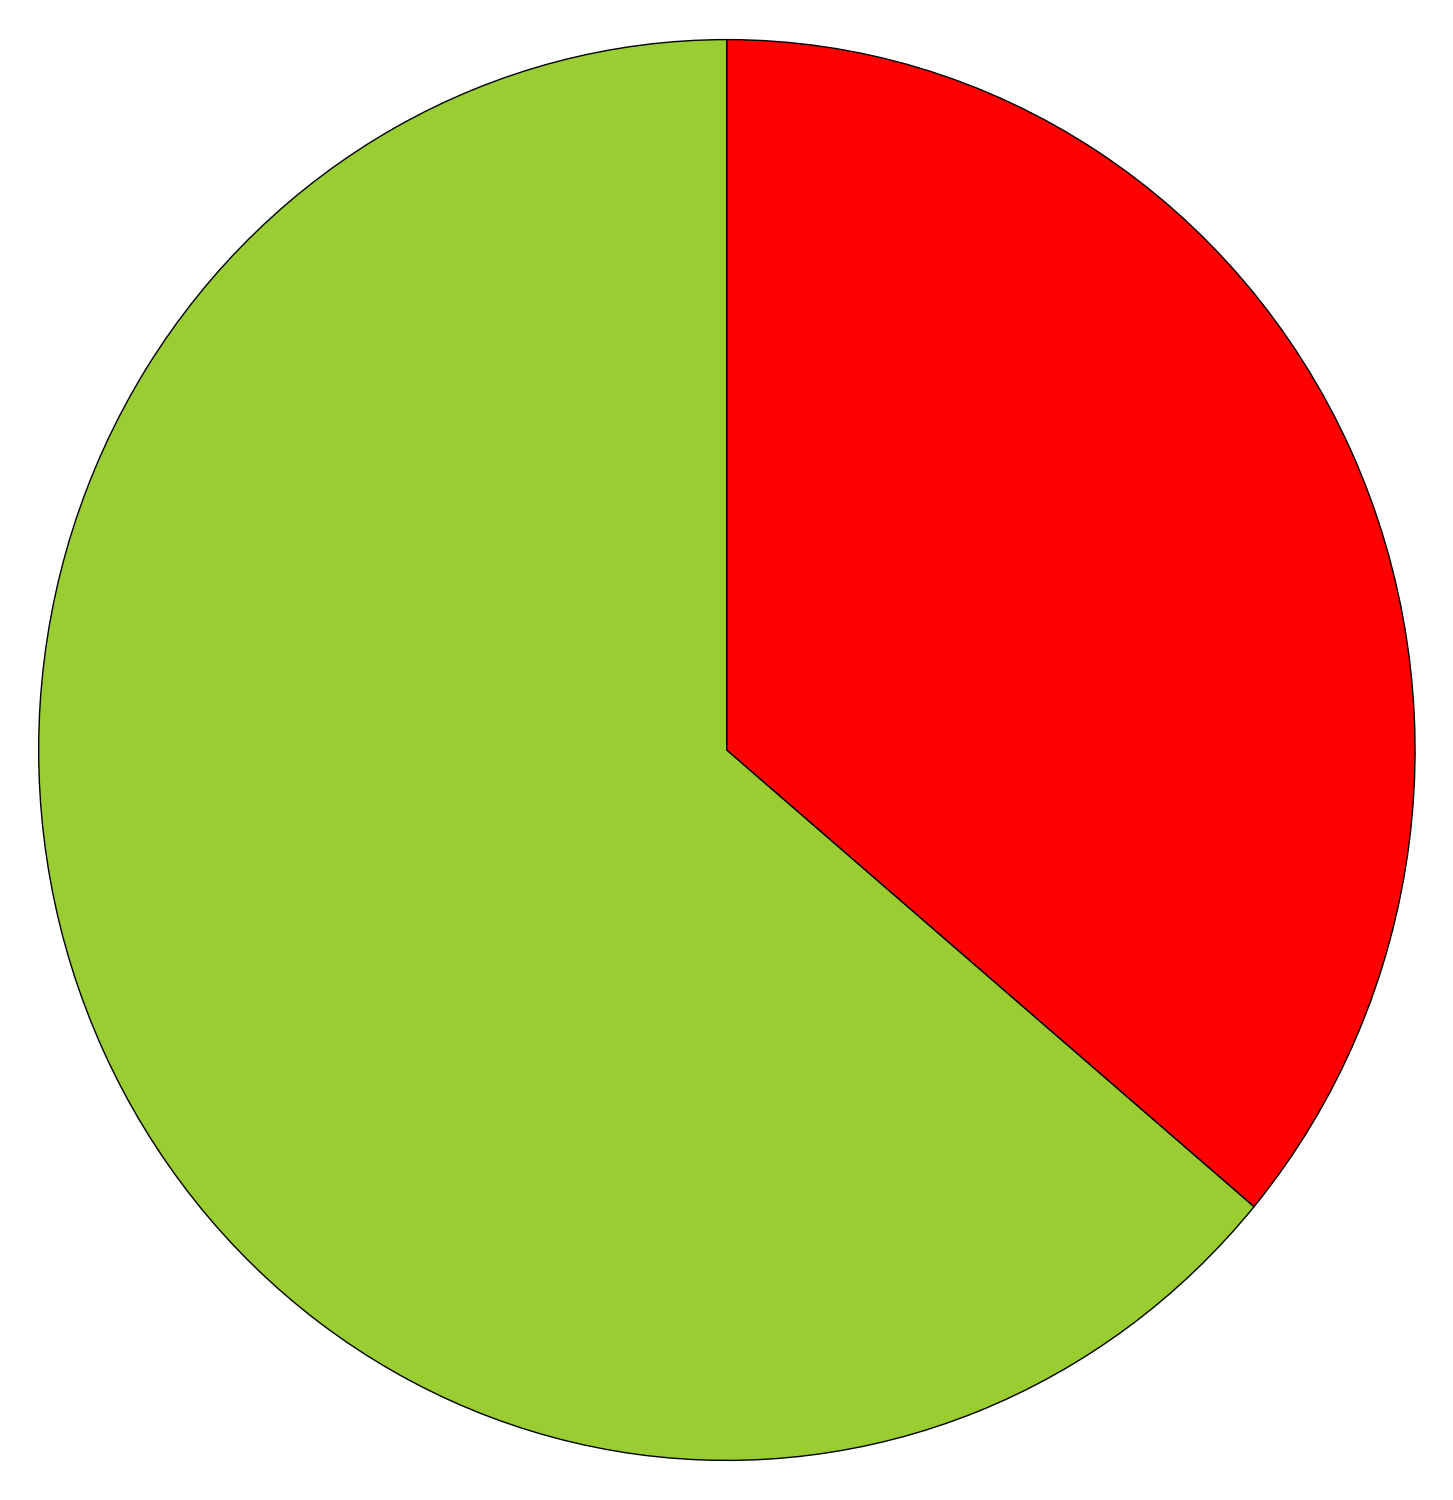
\includegraphics[width=\textwidth]{arousalasymzonesASM}
    \caption{Origin of the asymmetry features for arousal classification.\label{arousalasymzonesASM}}
  \end{subfigure}
\hfill
  \begin{subfigure}[b]{.4\textwidth}
    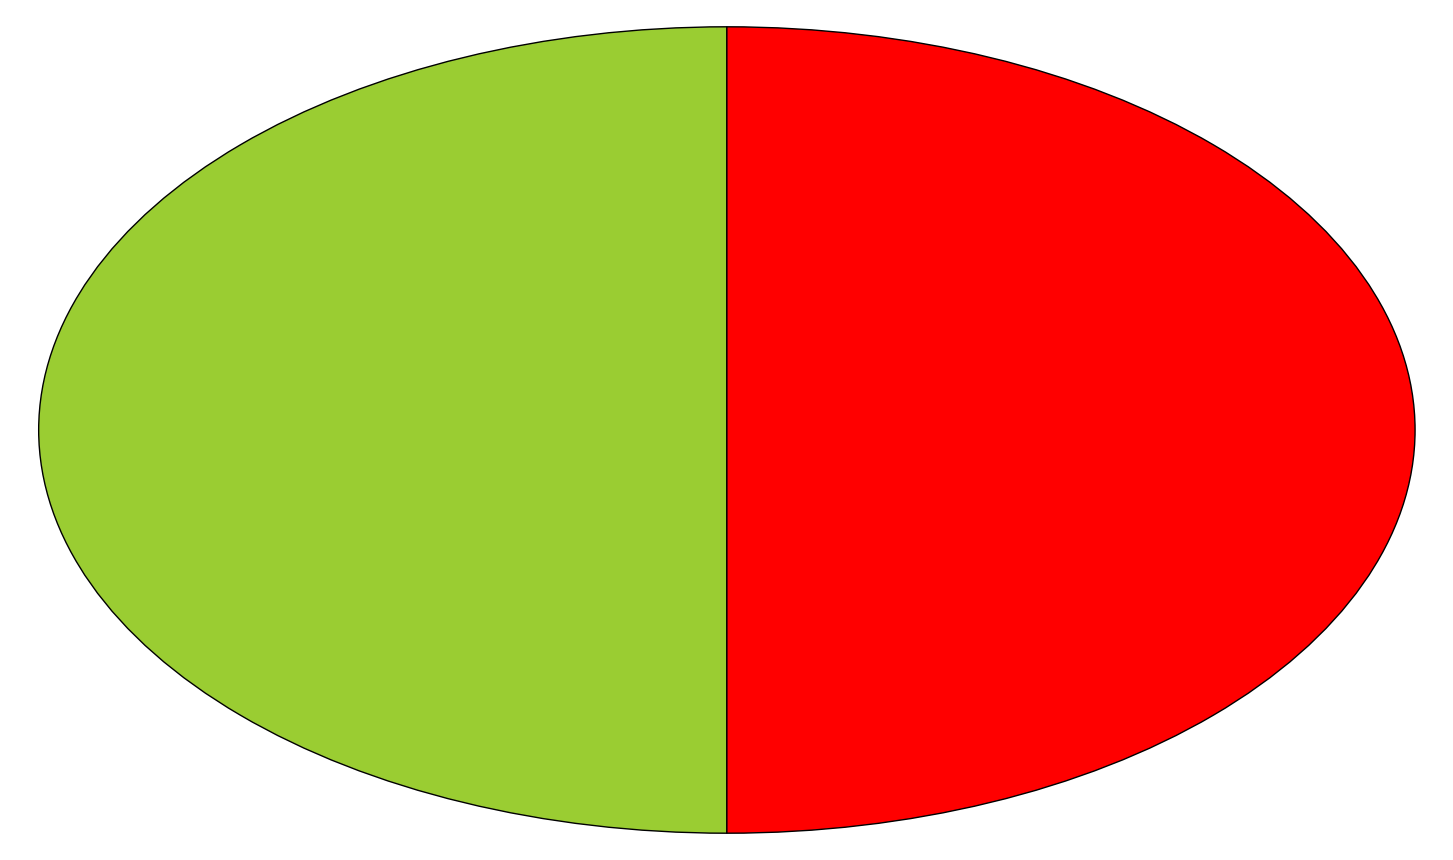
\includegraphics[width=\textwidth]{valenceasymzonesASM}
    \caption{Origin of the asymmetry features for valence classification.\label{valenceasymzonesASM}}
  \end{subfigure}
\\
  \begin{subfigure}[b]{.4\textwidth}
    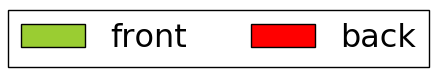
\includegraphics[width=\textwidth]{ASMlegend}
    \caption{The corresponding zone for each color.\label{ASMlegend}}
  \end{subfigure}
\end{figure}

For the DASM and RASM features, it is clear that the asymmetry should be measured at the front of the scalp for arousal. For valence however, features are selected from the front and the back of the scalp. This is in contradiction with the literature, most studies suggest that the frontal asymmetry of alpha power is most valuable.

\npar

The caudality features also measure asymmetry, but between a frontal and posterior channel. Here, the channel pairs were grouped in three groups: left, right and Fz/PZ, since the Fz/Pz channel pair lies on the central line. The specific grouping is shown in Table \ref{CAUgroupTable} below.

%table
\begin{table}[H]
\centering
\caption{The region for each corresponding DASM and RASM channel pair\label{CAUgroupTable}.}
\begin{tabular}{ll|ll}
\textbf{Channel pair} & \textbf{Group} & \textbf{Channel pair} & \textbf{Group} \\ \hline
FC5,CP5               & left           & FC6,CP6               & right          \\
FC1,CP1               & left           & FC2,CP2               & right          \\
F3,P3                 & left           & F4,P4                 & right          \\
F7,P7                 & left           & F8,P8                 & right          \\
Fp1,O1                & left           & Fp2,O2                & right          \\
Fz,Pz                 & Fz/Pz          &                       &                \\
\end{tabular}
\end{table}

\begin{figure}[H]
\centering
  \begin{subfigure}[b]{.4\textwidth}
    \includegraphics[width=\textwidth]{arousalasymzonesCAU}
    \caption{Origin of the asymmetry features for arousal classification.\label{arousalasymzonesCAU}}
  \end{subfigure}
\hfill
  \begin{subfigure}[b]{.4\textwidth}
    \includegraphics[width=\textwidth]{valenceasymzonesCAU}
    \caption{Origin of the asymmetry features for valence classification.\label{valenceasymzonesCAU}}
  \end{subfigure}
\\
  \begin{subfigure}[b]{.5\textwidth}
    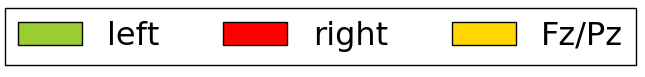
\includegraphics[width=\textwidth]{CAUlegend}
    \caption{The corresponding zone for each color.\label{CAUlegend}}
  \end{subfigure}
\end{figure}

For the arousal it seems that the caudality of the right of the brain might be of more interest. Valence uses caudality features from all over the brain.

\npar

These results indicate that for valence can be measured with channels from all over the scalp, while arousal seems to rely most on frontal channels.